\documentclass{aip-cp}

\usepackage[numbers,elide]{natbib}
\usepackage{fancybox}
\usepackage{shortvrb}
\MakeShortVerb\|

\usepackage{listings}
\usepackage[usenames]{color}
\definecolor{codecolor}{gray}{.9}
\definecolor{rlcolor}{cmyk}{0,1,0,0}
\lstset{basicstyle=\footnotesize\ttfamily,backgroundcolor=\color{codecolor},frameround=ffft,frame=single}%rulecolor=\color{rlcolor}
%%%%%%%

\newcommand\aipcls{\texttt{aip-cp} class}
\newtheorem{theorem}{Theorem}
\newcommand\BibTeX{\textsc{Bib}\TeX{}}
\begin{document}

\title{Author Guide for AIP Conference Proceedings:\endgraf
Setting Up Your \LaTeXe{} Files}

\author{AIP TeX Support}
\eaddress{tex@aip.org}


\maketitle

\begin{abstract}
This guide provides information on the various
options/functionalities available in \texttt{aip-cp} class with \LaTeX{}
for generating the papers for submission to AIP Conference Proceedings.
Commands that differ from the \texttt{article} class of standard \LaTeX{} interface, or that are
provided in addition to the standard interface, are explained in this
guide. This guide is not a substitute for the LATEX manual itself but should be used together with an introductory
  manual on \LaTeX{}, e.g., see Ref.~\cite{A-W:LLa94}.
\end{abstract}

\section{INTRODUCTION}

The \texttt{aip-cp} class is a \LaTeX{} document class for AIP Conference proceedings and other documents with similar layout requirements.
\texttt{aip-cp} class is primarily based on the default \texttt{article} class. This class
depends on the following packages for its proper functionality:
\begin{itemize}
\item{}\texttt{natbib.sty} for citation processing;
\item{}\texttt{graphicx.sty} for graphics inclusion;
\item{}\texttt{txfonts.sty} optional font package, if document is to be formatted with Times and compatible math fonts;
\item{}\texttt{hyperref.sty} optional packages if hyperlinking is required in the document.
\end{itemize}
These packages are part of any standard \LaTeX{} installation.
Furthermore, users are free to make use of AMS math packages such as
|amsmath.sty|, |amsthm.sty|, |amssymb.sty|, |amsfonts.sty|, etc., if they
want to. Authors can use these packages as per their specific requirements.

The class provides essentially the same markup as
implemented by \LaTeX{} standard article class. In
addition to this, it implements the following:
\begin{itemize}
\item{}extended set of front matter commands,
\item{}allows mixing column and page-wide floats without getting the numbering out of sync,
\item{}footnotes will appear below bottom floats,
\item{}extended set of citation commands if the natbib system is installed,
\item{}support for table notes.
\end{itemize}

\section{USING THE \texttt{aip-cp} CLASS}

If the file \texttt{aip-cp.cls} is not already in the appropriate system directory for \LaTeX{} files,
either place the file there or copy it to your working directory. In
order to use the \texttt{aip-cp} class, replace \texttt{article} by \texttt{aip-cp} in the \texttt{\string\documentclass} command at the beginning of your document:
\begin{verbatim}
\documentclass{article}
\end{verbatim}
is replaced by
\begin{verbatim}
\documentclass{aip-cp}
\end{verbatim}
In general, the following standard document style options should not be used with the \texttt{aip-cp} class:
\begin{enumerate}
\item{}10pt, 11pt, 12pt � unavailable;
\item{}twoside (no associated style file) � twoside is the default;
\item{}fleqn, leqno, titlepage � should not be used.
\end{enumerate}

\subsection{Additional Document Class Options}
Please place any additional command definitions at the very start of
the LATEX file i.e., before the |\begin{document}|. For example, user-defined |\def| and |\newcommand| commands that define macros for technical expressions should be placed here. Other author-defined macros should be kept to a mininum.

The following additional class options are available with the \texttt{aip-cp} class file:

\begin{itemize}
\item{}\textbf{Paper Size}---\texttt{aip-cp} class fully supports both the US letter (8.5in $\times$ 11in) and
A4 (210mm $\times$ 297mm) paper sizes.
\begin{itemize}
\item{}\texttt{letterpaper:} Instruct the system to generate the output on US letter sized paper (default).
\item{}\texttt{4apaper:}  Instruct the system to generate the output on A4 sized paper.
\end{itemize}
Changing the paper size in the standard conference modes will not
alter the typesetting of the document---only the margins will be
affected.  

\item{}\textbf{Citations and Bibliography}---The \texttt{aip-cp}
class provides the following options for Citations and Bibliography:
\begin{itemize}
\item{}\texttt{author-numerical (default):} This optiopn generates
the numbered bibliography in text as well as at the end of the papers.
\item{}\texttt{author-year:} With this option, system will generate
the output in author/year scheme. In combination with
\texttt{natbib.sty}, the \texttt{aip-cp} class also provides some
expended commands.
\end{itemize}

\item{}\textbf{Heading numbers}---Heading numbers can be turned on or off with the following two options:
\begin{itemize}
\item{}\texttt{numberedheadings:} Headings are numbered.
\item{}\texttt{unnumberedheadings:} Headings are unnumbered
(default). 
\end{itemize}

\item{}All options of \texttt{article.cls} can be used with this document class.
\end{itemize}

\subsection{Front matter}

\noindent\Ovalbox{\verb"\title{The Title Goes Here with Each Initial Letter Capitalized}"}\\

All the authors appear as single group with footnote marker for the
affiliation's appearing in a separate group. Below is an example of
the same:\\

\begin{lstlisting}
\author[aff1]{Author's Name\corref{cor1}}
\eaddress[url]{http://www.aptaracorp.com}

\author[aff2,aff3]{Author's Name}
\eaddress{anotherauthor@thisaddress.yyy}

\affil[aff1]{Replace this text with an author's affiliation
   (use complete addresses). Note the use of superscript ``a'' to indicate
   the author's e-mail address below. Use b), c), etc. 
   to indicate e-mail addresses for more than 1 author.}
\affil[aff2]{Additional affiliations should be indicated by 
  superscript numbers 2, 3, etc. as shown above.}
\affil[aff3]{You would list an author's second affiliation here.}

\corresp[cor1]{Corresponding author: your@emailaddress.xxx}
\end{lstlisting}

\ \\
Supported commands will be |\corresp[<label>]{corresponding text}|
with optional argument to generate number, |\corref{<label>}| will
generate cross-ref for author, |\eaddress{e-mail}| is for providing
author's email, another variant for |\eaddress| is with optional
argument to specify the author's homepage as\break
|\eaddress[url]{http://www.aip.org}|

\pagebreak

\noindent\Ovalbox{\verb"\maketitle"}\\

This command inserts the actual front matter data. It has to follow the
above declarations before the |abstract| environment.\\

\noindent\Ovalbox{\verb"\begin{abstract}"}\\

At the beginning of your article, the title should be generated in the usual
way using the \maketitle command. The abstract should be enclosed
within an abstract environment. The coding for the same is as follows:\\

\begin{lstlisting}
\maketitle
\begin{abstract}
We study
.
.
\end{abstract}
\end{lstlisting}


\subsection{Cross-references}

For cross-references of figures, tables, equations, etc., the pair
of commands \verb"\label" and \verb"\ref" is available. Since the usage
of these two commands is exactly the same as that in the standard
\LaTeX, we leave the explanation about \verb"\label" and \verb"\ref" to
adequate instructions of \LaTeX. Since headings in this layout do not carry numbers they cannot be referenced either.


\subsection{Lists}

The \texttt{aip-cp} supports all standard list environments like
|itemize|, |enumerate|, etc.\\

\begin{lstlisting}[morekeywords={Bullet,List},keywordstyle=\color{blue}\bfseries]
Bullet List
\begin{itemize}
\item first bulleted item
\item second bulleted item
\end{itemize}
\end{lstlisting}

\begin{itemize}
\item first bulleted item
\item second bulleted item
\end{itemize}

\begin{lstlisting}[morekeywords={Numbered,List},keywordstyle=\color{blue}\bfseries]
Numbered List
\begin{enumerate}
\item first numbered item
\item second numbered item
\end{enumerate}
\end{lstlisting}

\begin{enumerate}
\item first numbered item
\item second numbered item
\end{enumerate}

\subsection{Floating Bodies}

Most publications contain figures and tables, these elements
need special treatment, because they cannot be broken across pages.
The solution to this requirement is to �float� any figure or table that does not
fit on the current page to a later page, while filling the current page with
body text.

\LaTeX{} offers two environments for floating bodies: one for figures
and one for tables. To take full advantage of these two environments, it is
important to understand approximately how \LaTeX{} handles floats
internally.

\subsection{Figures}

The \texttt{aip-cp} class will address the positioning of your figures and therefore you should
not normally use the optional positional qualifiers on the figure environment that would
override these decisions.

Figure captions should be \textit{below} the figure itself, therefore the \verb"\caption" command
should appear after the figure or space left for an illustration. For example, Figure~\ref{fig:a} is
produced using the following commands:\\

\begin{lstlisting}
\begin{figure}
  \centerline{%
  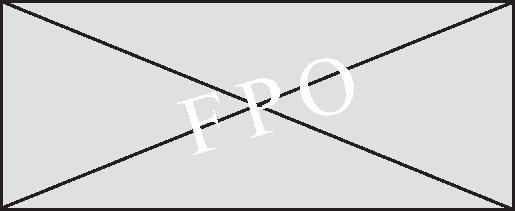
\includegraphics
   [width=.75\textwidth]{art/fig_1}}
 \caption{While it is possible to extend our within-household model to
include multiple infecteds, this would be very tedious.}
 \label{fig:a}
\end{figure}
\end{lstlisting}

\begin{figure}
  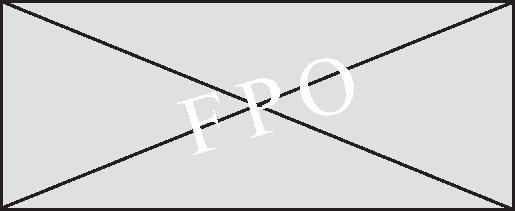
\includegraphics[width=.5\textwidth]{art/fig_1}
 \caption{While it is possible to extend our within-household model to
include multiple infecteds, this would be very tedious.}
 \label{fig:a}
\end{figure}

For cross-referencing of figures using the \verb"\label" and
\verb"\ref" commands is encouraged. For example, in referencing
Figure~\ref{fig:a} above, we used Figure\verb"~\ref{fig:a}". 

\subsubsection{Graphics Support}

Support for including and manipulating graphics is provided as the
standard \LaTeX{} \texttt{graphicx} package is automatically loaded by
the \texttt{aip-cp} class.

Figures can be scaled using the \verb"[width=...]" option of the \verb"\includegraphics" command. For example,
\verb"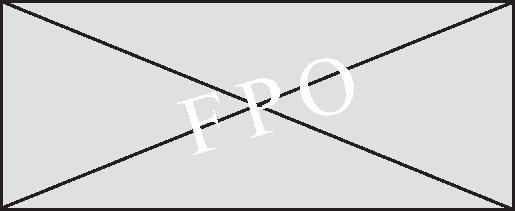
\includegraphics[width=.5\textwidth]{art/fig_1}". One
could also provide the absolute dimensions (e.g.,
\verb"width=3in").

\subsection{Tables}

The \texttt{aip-cp} class file will cope with most positioning of your tables and you should not normally
use the optional positional qualifiers on the table environment which would override these decisions.
Table captions should be at the top, therefore the \verb"\caption" command should appear above the body
of the table.

\subsubsection{Table Headings}

\noindent\Ovalbox{\verb"\tch{cols}{h-pos}{v-pos}{heading text}"}\\

To ease the production of tables, the command |\tch| is provided
which is essentially an abbreviation for a |\multicolumn| command
that additionally boldens its text argument. I.e., |cols| specifies the number of columns the |heading text| should span
and |h-pos| defines the horizontal positioning of the text of the column(s), e.g., |l|, |r|, |c|, or |p{...}|.  In contrast to a simple
|\multicolumn| command the |heading text| can be split vertically by using |\\| to denote the line breaks.  The |v-pos| argument should contain either |t|, |c|, or |b| denoting the vertical placement
of the text in relation to other cells of that row. It is relevant if the |heading text| consists of more than one line.
This demonstrates the use of this command.

\subsubsection{Table Notes}

\noindent\Ovalbox{\verb"\tablenote[t1n1]{Table note text}"}\\

\noindent Command to produce a note to the table. It can be used
after the |tabular| environment or table body. The command contains the table note text with optional label (id) to produce the numbered note. If the number is not required, omit the |<label>| and use |\tablenote{Tablenote text}|. The default number of table note is $*,\dagger,\ddagger,\mathsection,\mathparagraph,\|,**,\dagger\dagger$, etc.\\


\noindent\Ovalbox{\verb"\tabnoteref{t1n1}"}\\

\noindent|\tabnoteref| command is used for cross-referencing of the table note and should be used in the table body. The |<label>| will determine the referencing number/symbol. Multiple |labels| can be used separated with comma as\break
 |\tabnoteref{t1n1,t2n2}|. Please note that every |<label>| should be unique for correct cross-referencing.\\

\noindent |\hline| can be used for horizontal lines to separate the |caption|, |table head|, |table body|, and |table note| eachother respectively.\\


\noindent Typically the body of the environment would consist of a
|tabular| environment responsible for producing the actual table including the table and stub headers.\\

An example showing the use of all commands described above is shown in Table~\ref{tab:a}.\\

As with figures, cross-referencing of tables is also encouraged. For example, we would reference Table~\ref{tab:a} using \verb"Table~\ref{tab:a}". Label of Table must be given after the \verb"\caption" for correct numbering in the cross-referecing.\\

For example, Table~\ref{tab:a} is produced using the following coding.\\

\begin{lstlisting}
\begin{table}
\caption{Average turnover per shop: by type of retail organisation
\label{tab:a}}
\begin{tabular}{lcccc}
\hline
  & \tch{1}{c}{b}{Single\\ outlet\tabnoteref{t1n1}}
  & \tch{1}{c}{b}{Small\\ multiple}  
  & \tch{1}{c}{b}{Large\\ multiple}
  & \tch{1}{c}{b}{Total} \\
\hline
1982 & 98  & 129 & 620    & 847\\
...
1998 & 200 & 300 & 1500\tabnoteref{t1n2}  & 2000\\
\hline
\end{tabular}
\tablenote{This is an example of unnumbered tablenote entry}
\tablenote[t1n1]{This is an example of first numbered tablenote entry}
\tablenote[t1n2]{This is an example of second numbered tablenote entry}
\end{table}
\end{lstlisting}


\subsection{Landscaping pages}

If a table/figure is too wide to fit the standard measure, it may be turned, with its caption, to 90 degrees. Landscape tables/figures cannot be produced directly using the \texttt{aip-cp} class file because LATEX itself cannot turn the page, and not all device drivers provide such a facility. The following procedure can be used to produce such pages.

\pagebreak

Use the package |rotating| in your document and change the coding from\\

\begin{lstlisting}[morekeywords={Figures,Tables},keywordstyle=\color{blue}\bfseries]
Figures
        \begin{figure}....\end{figure}

\begin{sidewaysfigure}....\end{sidewaysfigure}

Tables
        \begin{table}....\end{table}
\begin{sidewaystable}....\end{sidewaystable}
\end{lstlisting}


\subsection{Long tables}

Tables which are longer than one page cannot be placed into a \verb"table" environment as floats cannot have a size larger than a page. Such tables are supported by the standard \LaTeX{} package \verb"longtable" written by David Carlisle. Refer to the package documentation for the syntax description.

\subsection{Footnote}
\LaTeX{} provides \verb"\footnote" command to generate the footnoote.\footnote{This is an example of footnote.} It can be produced by\\

\begin{lstlisting}
\footnote{This is an example of footnote.}
\end{lstlisting}

\begin{table}
\caption{Average turnover per shop: by type  of retail organisation\label{tab:a}}
\centering\begin{tabular}{lcccc}
\hline
  & \tch{1}{c}{b}{Single\\ outlet\tabnoteref{t1n1}}  & \tch{1}{c}{b}{Small\\ multiple}  & \tch{1}{c}{b}{Large\\ multiple}  & \tch{1}{c}{b}{Total}   \\
\hline
1982 & 98 & 129 & 620    & 847\\
1987 & 138 & 176 & 1000  & 1314\\
1991 & 173 & 248 & 1230  & 1651\\
1998 & 200 & 300 & 1500\tabnoteref{t1n2}  & 2000\\
\hline
\end{tabular}
\tablenote{This is an example of unnumbered tablenote entry}
\tablenote[t1n1]{This is an example of first tablenote entry}
\tablenote[t1n2]{This is an example of second tablenote entry}
\end{table}

\subsection{Typesetting mathematics}

\LaTeX{} allows two writing modes for mathematical expressions: the \textbf{inline mode} and the \textbf{display mode}. The first one is used to write formulas that are part of a text. The second one is used to write expressions that are not part of a text or paragraph, and are therefore put on separate lines.

\subsubsection{Inline Mathematics}
To put your equations in inline mode use one of these delimiters:
\verb"\( \)" or \verb"$ $".

\subsubsection{Displayed Mathematics}
The \texttt{aip-cp} class supports all the standard features in
this respect. \texttt{aip-cp} class set displayed mathematics
with center to the text width. The \textit{displayed} mode has two
versions: numbered and unnumbered. Below are examples for both: 


\begin{lstlisting}[morekeywords={Unumbered,Equation},keywordstyle=\color{blue}\bfseries]
Unumbered Equation
\[
  \phi_{d_{f}} (\mathbf{r}) = \sum_{i} d^{f}_{i} \phi_{i} (\mathbf{r}).
\]
\end{lstlisting}

\[
  \phi_{d_{f}} (\mathbf{r}) = \sum_{i} d^{f}_{i} \phi_{i} (\mathbf{r}).
\]

\begin{lstlisting}[morekeywords={Numbered,Equation},keywordstyle=\color{blue}\bfseries]
Numbered Equation
\begin{equation}
R_K^{F/J} (\rho) \approx \frac{1}{\mu} \left[  H_K + \frac{\rho}{2(1-\rho)}                           
\left(\sum_{i=1}^K \frac{1}{i-\rho} + (1-2 \rho)\sum_{i=1}^K \frac{1}{i(i-\rho)}
\right) \right].
\end{equation}
\end{lstlisting}

\begin{equation}
R_K^{F/J} (\rho) \approx \frac{1}{\mu} \left[  H_K + \frac{\rho}{2(1-\rho)}                           
\left(\sum_{i=1}^K \frac{1}{i-\rho} + (1-2 \rho)\sum_{i=1}^K \frac{1}{i(i-\rho)}
\right) \right].
\end{equation}

\subsection{Acknowledgments}
These should appear at the close of your paper, just before the list of references. Use the acknowledgments environment, e.g.,

\begin{verbatim}
\section{ACKNOWLEDGMENTS}
The research and writing of this work was partially carried out...
\end{verbatim}


\subsection{Bibliography}

Referring to other articles, books, etc.\ can be done using the |\cite| command of standard \LaTeX{}. The list of references itself can either be produced using standard \LaTeX{} methods or using \textsc{Bib}\TeX.
	
For this, we recommend the use of |natbib.sty| after the |\documentclass{aip-cp}| declaration. The \texttt{natbib} system has two basic citation commands, |\citet| and |\citep| for \emph{textual} and \emph{parenthetical} citations, respectively. There also exist the starred versions |\citet*| and |\citep*| that print the full author list, and not just the abbreviated one. All of these may take one or two optional arguments to add some text before and after the citation. The following table shows some examples:\\[.1in]

\begin{tabular}{@{}l@{\quad$\Rightarrow$\quad}l@{\quad$\Rightarrow$\quad}l}
\hline
\tch{1}{l}{b}{Commands} & \tch{1}{l}{b}{Author-Year Style} & \tch{1}{l}{b}{Numerical Style}\\
\hline
  |\citet{jon90}| & Jones et al. (1990) & Jones et al. [21]\\[.1in]
  |\citet[chap.~2]{jon90}| & Jones et al. (1990, chap.~2) & Jones et al. [21, chap.~2]\\[.1in]
  |\citep{jon90}| & (Jones et al., 1990)& [21]\\[.1in]
  |\citep[chap.~2]{jon90}| & (Jones et al., 1990, chap.~2) & [21, chap.~2]\\[.1in]
  |\citep[see][]{jon90}| & (see Jones et al., 1990) & [see 21]\\[.1in]
  |\citep[see][chap.~2]{jon90}| & (see Jones et al., 1990, chap.~2) & [see 21, chap.~2]\\[.1in]
  |\citet*{jon90}| & Jones, Baker, and Williams (1990) & [21]\\[.1in]
  |\citep*{jon90}| & (Jones, Baker, and Williams, 1990) \\[.1in]
\hline
\end{tabular}\\


For more information regarding these commands, the authors can refer to the documentation of |natbib| package.


\subsubsection{Bibliography Produced Manually}

In \texttt{aip-cp} class, |\begin{thebibliography}{} ... \end{thebibliography}| command
can be used to produce bibliography. The coding is as follows:\\

\begin{lstlisting}
\begin{thebibliography}{1}
\bibitem{man:aipproceed}
American Institute of Physics, \emph{Conference Proceedings: Instructions for
  Camera Ready Manuscripts}, Feb 2000.

\bibitem{man:Daly99a}
P. Daly, \emph{Natural Sciences Citations and References
  (Author--Year and Numerical Schemes)},
  1999, distributed as \texttt{natbib.dtx} with the \texttt{natbib} software.

\bibitem{man:Daly99b}
P. Daly, \emph{Reference sheet for \texttt{natbib} usage},
  1999, distributed as \texttt{natnotes.tex} with the  \texttt{natbib}
  software.
\end{thebibliography}
\end{lstlisting}

\subsubsection{Bibliography Produced Using \textsc{Bib}\TeX}

The \aipcls{} is accompanied by \BibTeX{} style files which can be used
to produce compliant reference lists from \BibTeX{} database
files. To use \BibTeX{} one first has to run the source file through
\LaTeX{} then run \BibTeX{} and then rerun \LaTeX{} twice to get all
references resolved. \BibTeX{} is described in more detail in Appendix
B of Ref.~\cite{A-W:LLa94} and in Chapter~13 of Ref.~\cite{A-W:MG04}.\\

\noindent\Ovalbox{\verb"\bibliographystyle{style-name}"}\\

This declaration specifies to \BibTeX{} that the style
\texttt{style-name} should be used. It can be placed anywhere within the
document but is usually positioned directly in front of the command
described below.

For a AIP Conference Proceddings we recommend the use of
|aipnum-cp.bst| provided with this packet. This bibliograpgy style
generates numbered style references in the required format.\\

\noindent\Ovalbox{\verb"\bibliography{bib-list}"}\\

This command denotes the position where the reference list produced by
\BibTeX{} will be included in the document. The \texttt{bib-list} is a
comma separated list of \BibTeX{} database files.

\begin{thebibliography}{1}

\bibitem{man:aipproceed}
American Institute of Physics, \emph{Conference Proceedings: Instructions for
  Camera Ready Manuscripts}, Feb 2000.

\bibitem{man:Daly99a}
P. Daly, \emph{Natural Sciences Citations and References
  (Author--Year and Numerical Schemes)},
  1999, distributed as \texttt{natbib.dtx} with the \texttt{natbib} software.

\bibitem{man:Daly99b}
P. Daly, \emph{Reference sheet for \texttt{natbib} usage},
  1999, distributed as \texttt{natnotes.tex} with the  \texttt{natbib}
  software.

\bibitem{A-W:KD04}
H.~Kopka and P.~Daly, \emph{Guide to {\LaTeX}}, Tools and
  Techniques for Computer Typesetting, Addison-Wesley, Boston, Massachusetts,
  2004, 4 edn., ISBN 0-321-17385-6.

\bibitem{A-W:MG04}
F.~Mittelbach and M.~Goossens, \emph{The {\LaTeX} Companion}, Tools and
  Techniques for Computer Typesetting, Addison-Wesley, Boston, Massachusetts,
  2004, 2 edn., ISBN 0-201-36299-6, with Johannes Braams, David Carlisle, and
  Chris Rowley.

\bibitem{A-W:GMR97}
M.~Goossens, S.~Rahtz, and F.~Mittelbach, \emph{The {\LaTeX} Graphics
  Companion}, Tools and Techniques for Computer Typesetting, Addison-Wesley,
  Reading, Massachusetts, 1997, ISBN 0-201-85469-4.

\bibitem{A-W:LLa94}
L.~Lamport, \emph{{\LaTeX:} A Document Preparation System}, Addison-Wesley,
  Reading, Massachusetts, 1994, \nobreak{second}~edn.

\end{thebibliography}



\end{document}

